\documentclass[conference]{IEEEtran}
\IEEEoverridecommandlockouts
\usepackage{cite}
\usepackage{amsmath,amssymb,amsfonts}
\usepackage{graphicx}
\usepackage{booktabs}
\usepackage{url}
\usepackage{siunitx}
\usepackage{pgfplots}
\pgfplotsset{compat=1.16}
\providecommand{\degree}{\ensuremath{^\circ}}

\begin{document}

\title{A Held-Out Audit of Nonlinear Filters for\\
Light-Level Geolocation of a Juvenile White Shark}

\author{\IEEEauthorblockN{Viviane Solomon}
\IEEEauthorblockA{\textit{Harvey Mudd College}\\
Claremont, CA, USA}}

\maketitle

\begin{abstract}
Pop-up archival transmitting (PAT) tags infer animal position from the timing of
sunrise and sunset. The measurement is well conditioned in longitude and nearly
singular in latitude near an equinox, which makes it a useful stress test for
nonlinear filtering. I build an extended Kalman filter, an unscented Kalman
filter, a bootstrap particle filter, two smoothers and a grid HMM for a 137-day
juvenile white shark (\emph{Carcharodon carcharias}) record, and I score them
against 122 Argos satellite fixes obtained for the same animal.
The contribution is not an error number; it is an audit. I hold out the final
30 days of the ground truth, never using it for any modelling or tuning
decision, and I repeat every stochastic run over ten seeds.
Four results follow. First, the best configuration I built reaches
$117$\,\si{\km} median error on the window I tuned on and $544$\,\si{\km} on the
held-out window, where the proprietary GPE3 smoother reaches
$118$\,\si{\km}: the headline was a tuning-window number.
Second, seed-to-seed spread is $29$--$90$\,\si{\km}, far larger than the
$1$--$5$\,\si{\km} steps an earlier ablation ladder reported, so those steps were
noise. Third, across $75$ pipeline variants, tuning-window rank predicts
held-out rank only weakly (Spearman $\rho=+0.30$), and the variant that looks
best while tuning ranks $54$th of $75$ when finally tested. Fourth, the failure
has an identifiable physical cause, and a one-parameter fix chosen without ever
touching the held-out data raises tuning-window $1\sigma$ coverage from
$22\%$ to $38\%$ while leaving held-out error unchanged to worse. I report the
fix because it failed, and the one estimator that does generalise is the one I
did not write.
\end{abstract}

\begin{IEEEkeywords}
state estimation, particle filter, unscented Kalman filter, animal telemetry,
model validation, overfitting, reproducibility
\end{IEEEkeywords}

\section{Introduction}
A PAT tag carries no receiver. It records light, pressure and temperature, and
position must be inferred afterwards from the astronomy of the light curve.
Local apparent noon gives longitude directly and robustly. Latitude comes only
from day length, and
$\partial(\text{day length})/\partial(\text{latitude}) \rightarrow 0$ at an
equinox, so for weeks around it the inverse problem is locally rank deficient in
latitude. This deployment runs straight through the March 2008 equinox.

That makes it a good test case for nonlinear filtering, and the second tag on
the same animal makes it a rare one: the Argos fixes give an independent answer
that the light data never sees. Most light-level geolocation papers validate
against simulation or against a single reference track. Here there is a real,
external, irregularly sampled ground truth.

This paper is deliberately an audit rather than a method paper. An earlier
version of this pipeline reported a best median error near $119$\,\si{\km} and a
ladder of incremental improvements. Everything in Section~\ref{sec:proto} was
added afterwards, and most of what the ladder claimed did not survive it. The
useful output is therefore a set of statements about what the data can and
cannot resolve, and a short list of process errors that produced the original
over-claim.

\section{Data}
\subsection{Tag record}
Deployment \texttt{07\_05} is a juvenile white shark tagged off central
California on 5 February 2008. The archival tag was physically recovered, so the
full-resolution record is available rather than the summarised transmission:
light level, pressure and temperature at $10$-second to $1$-minute cadence over
$137$ days. The animal left the shelf and moved south and offshore, ending near
the southern Gulf of California.

Twilight events are extracted in two ways. The manufacturer's LightLoc
processing yields $251$ twilight times, $241$ after quality control. A
re-extraction directly from the raw light curves yields $228$ events with an
explicit depth of detection attached to each, which Section~\ref{sec:recal}
uses.

\subsection{Ground truth}
A SPOT tag on the same animal returned $122$ Argos fixes between
15 February and 15 June 2008. Location classes are $3$ ($n=3$), $2$ ($20$),
$1$ ($42$), $0$ ($24$), A ($16$) and B ($16$). I assign them nominal
one-sigma radii of $0.25$, $0.5$, $1.5$, $10$, $3$ and $9$\,\si{\km}
respectively; classes 0, A and B are unquoted by Argos, so these are the
empirical marine-vertebrate values rather than anything the system guarantees.

The Argos track is the only ground truth used anywhere in this paper. It is
never an input to any estimator.

\begin{figure}[t]
\centering
\includegraphics[width=\columnwidth]{figs/05_map_all_methods}
\caption{Argos ground truth (black) and estimated tracks. The animal leaves the
California shelf, crosses the equinox offshore, and ends in the southern Gulf of
California.}
\label{fig:map}
\end{figure}

\begin{figure}[t]
\centering
\includegraphics[width=\columnwidth]{figs/07_equinox}
\caption{Sensitivity of day length to latitude through the deployment. The
derivative passes through zero at the March equinox, where latitude is
unobservable from day length at any noise level.}
\label{fig:equinox}
\end{figure}

\section{Observation and Motion Models}
\subsection{Twilight timing}
For a twilight event at time $t$ of kind $k \in \{\text{dawn},\text{dusk}\}$, the
predicted event time is obtained by solving for the instant at which the solar
elevation equals a threshold $h_0^{(k)}$. The threshold is not the geometric
horizon: it absorbs sensor response, cloud, and the fact that the tag may be at
depth when the threshold is crossed. I model it as
\begin{equation}
h_0^{(k)}(z) = h_0^{(k)} + \beta \log(1+z),
\label{eq:h0}
\end{equation}
with $z$ the depth in metres at which the twilight was recorded. The residual is
taken in minutes and given a Student-$t$ likelihood with $\nu=4$ degrees of
freedom, which matters more than any other modelling choice here
(Section~\ref{sec:matched}).

Two calibrations of \eqref{eq:h0} appear in this paper. The first is frozen on the
LightLoc times in the calibration window and gives
$h_0^{\text{dawn}}=-9.91\degree$, $h_0^{\text{dusk}}=-0.29\degree$ and
$\beta=+0.89$ per log-metre, with per-branch residual standard deviations of
$12.88$ and $10.43$ minutes. The second refits the same form on the raw-light
times and gives $h_0^{\text{dawn}}=-5.56\degree$,
$h_0^{\text{dusk}}=-5.88\degree$ and $\beta=+0.0085$, with a residual RMS of
$4.80$ minutes. The second looks much better and behaves much worse;
Section~\ref{sec:recal} is about that.


\begin{figure}[t]
\centering
\includegraphics[width=\columnwidth]{figs/04_calibration_residuals}
\caption{Calibration-window twilight residuals after fitting \eqref{eq:h0} on
the LightLoc times. The fit is unbiased on the window it was fitted to, which is
the point: nothing here predicts the behaviour in Table~\ref{tab:resid}.}
\label{fig:cal}
\end{figure}

\subsection{Sea-surface-temperature aiding}
Daily $0.25\degree$ optimally interpolated SST is compared with the tag's
shallowest daily temperature, and the resulting log-likelihood is added to the
twilight term. The point of SST is not that it is accurate. It is that its
information is orthogonal to day length, so it carries latitude through the
equinox where the light data cannot. In March alone it moves the particle
filter from $522$ to $109$\,\si{\km} median error.

\subsection{Seafloor-depth aiding}
Where the tag's maximum daily depth exceeds the ETOPO seafloor depth at a
candidate position, that position is impossible. This enters as
$\log\Phi\!\left((d_{\max}(p)-z)/\sigma_B\right)$ with $\sigma_B=150$\,\si{\m},
plus a finite land penalty. It is a hard, highly informative constraint, and it
makes the posterior strongly multimodal, which is why the choice of point
estimate stops being innocent.

\subsection{Motion model}
The state is $x=[\varphi,\lambda,v_E,v_N]$ with a damped random walk in velocity,
\begin{equation}
\dot v = -v/\tau + w, \qquad \tau = 3\ \text{days},
\end{equation}
and $\sigma_v$ set so the stationary speed distribution has a sensible mean for
a juvenile white shark. Positions are confined to a generous box
($15\degree$--$50\degree$\,N, $140\degree$--$105\degree$\,W).

\section{Estimators}
I implement, all on the same observation and motion models: a naive
event-by-event inversion as a floor; an EKF and a UKF with $3\sigma$ innovation
gating; Rauch--Tung--Striebel and unscented RTS smoothers for each; a bootstrap
particle filter with systematic resampling and roughening; a two-filter particle
smoother; a cloud-level fusion of two particle filters differing only in their
observation model; and a grid HMM over a $0.25\degree$ lattice. The proprietary
GPE3 hidden-Markov smoother supplied by the tag manufacturer is included as an
external reference; I did not implement it and cannot inspect it.

\section{Evaluation Protocol}
\label{sec:proto}
This section is the part of the paper I would read first, because every number
after it depends on it and none of it existed in the earlier version.

\subsection{Three windows}
The record is split once, by date, and never re-split:
\begin{itemize}
\item \textbf{Calibration}, up to 10 March 2008. The only window in which any
sensor parameter is fitted.
\item \textbf{Tuning}, 11 March to 15 May 2008. Every modelling decision,
hyperparameter and readout choice in this paper was made by looking at this
window. It contains $64$ truth-matched twilight events.
\item \textbf{Lockbox}, the final 30 days from 16 May 2008. Scored once per
configuration, after the configuration was frozen. It contains $20$ events.
\end{itemize}
Nothing is selected on the lockbox anywhere, including the one hyperparameter
introduced in Section~\ref{sec:fix}. Where a lockbox column appears next to a
selection rule, it is printed for the reader and was not available to the rule.

\subsection{Metrics}
Error is the great-circle distance between an estimate interpolated to an Argos
fix time and that fix, reported as a median over matched events; the median
rather than the mean because the naive inversion produces occasional
thousand-kilometre outliers that would otherwise dominate. Alongside it I report
$1\sigma$ coverage: the fraction of matched events at which the truth falls
inside the estimator's own reported standard deviation. Nominal coverage for a
Gaussian is $68\%$. An estimator that is wrong is usable; an estimator that is
wrong and confident is not.

\subsection{Monte Carlo repetition}
Every particle-based result is the mean over ten seeds, reported with its
standard deviation across seeds. This is the single cheapest change in the
paper and the one that invalidated the most prior conclusions.

\section{Results}
\subsection{Where the methods land}
Table~\ref{tab:main} gives median error on the full evaluation set and,
separately, on the tuning window and the lockbox. All rows use one scorer and
one set of matched events, so the columns are comparable.

Two things are worth reading off it immediately. The GPE3 smoother is better
than everything I built, at $72$\,\si{\km}, and that gap is not closed anywhere
in this paper. And the ordering of my own rows changes completely between the
tuning column and the lockbox column: the best tuning-window configuration
($84.9$\,\si{\km}) is nearly the worst lockbox configuration
($543.9$\,\si{\km}), while a plain EKF smoother is the best lockbox
configuration at $319$\,\si{\km}.

\begin{table}[t]
\caption{Median great-circle error (\si{\km}), one scorer and one matched event
set throughout. ``Tune'' and ``Lock'' are the tuning window and the held-out
final 30 days. GPE3 is the manufacturer's smoother, included as an external
reference.}
\label{tab:main}
\centering
\begin{tabular}{lrrr}
\toprule
Method & All & Tune & Lock \\
\midrule
Naive daily inversion               &  513.8 &  570.5 &  473.7 \\
Naive daily inversion, QC           &  478.8 &  487.0 &  473.7 \\
\midrule
EKF                                 &  347.2 &  285.2 &  413.0 \\
UKF                                 &  356.6 &  291.2 &  417.1 \\
PF, light + depth                   &  316.9 &  240.2 &  391.0 \\
EKF + RTS smoother                  &  285.7 &  169.4 &  359.0 \\
UKF + unscented RTS                 &  283.7 &  173.0 &  362.9 \\
EKF + RTS, QC events                &  279.9 &  169.5 &  \textbf{319.4} \\
\midrule
PF + SST                            &  198.4 &  114.9 &  498.4 \\
PF + SST, thinned 1/3\,d            &  186.1 &  129.2 &  473.1 \\
Grid HMM filter                     &  163.9 &  130.1 &  569.2 \\
PF + SST, two-filter smoother       &  155.2 &  112.2 &  422.2 \\
PF + SST + seafloor                 &  152.8 &  123.2 &  452.4 \\
Two-filter cloud fusion (my best)   &  117.4 &  \textbf{84.9} &  543.9 \\
\midrule
GPE3 HMM smoother (not mine)        &   72.0 &   71.1 &  118.4 \\
\bottomrule
\end{tabular}
\end{table}

\subsection{The headline was a tuning-window number}
The earlier version of this work quoted its best configuration at roughly
$119$\,\si{\km} and stopped there. That number survives re-running: the
two-filter cloud fusion scores $117.4$\,\si{\km} on the full evaluation window.
What does not survive is the interpretation. On the final 30 days the same
configuration scores $543.9$\,\si{\km}, against $118.4$\,\si{\km} for GPE3 on
exactly those days. The full-window figure is dominated by the tuning window,
which carries $64$ of the $84$ matched events, so quoting it as an accuracy is
close to quoting a training error.

\subsection{Seed noise sets the resolution floor}
Table~\ref{tab:head} repeats one configuration ten times at $120{,}000$
particles. The standard deviation across seeds is $29$\,\si{\km} on the full
window and $90$\,\si{\km} on the lockbox. The earlier ablation ladder reported
improvements of $1$--$5$\,\si{\km} per step and treated them as real. They are
an order of magnitude below this floor. Measuring the noise before building the
ladder would have removed most of the ladder.

\begin{table}[t]
\caption{Ten seeds of one configuration at $120{,}000$ particles, with and
without the threshold-bias state of Section~\ref{sec:fix}. Errors are medians in
\si{\km}; cov is $1\sigma$ coverage against the filter's own reported standard
deviation; $\bar{s}$ is the median reported standard deviation in the lockbox.}
\label{tab:head}
\centering
\begin{tabular}{lrrrrrr}
\toprule
 & All & Tune & Lock & cov$_\text{T}$ & cov$_\text{L}$ & $\bar{s}_\text{L}$ \\
\midrule
As published            & $408.1$ & $363.4$ & $532.4$ & $22\%$ & $9\%$ & $201$ \\
\quad $\pm$ seed sd     & $29.2$  & $31.0$  & $89.5$  &        &       &       \\
$+$ bias state          & $420.4$ & $358.1$ & $615.4$ & $38\%$ & $8\%$ & $205$ \\
\quad $\pm$ seed sd     & $17.7$  & $13.1$  & $35.0$  &        &       &       \\
\bottomrule
\end{tabular}
\end{table}


\begin{figure}[t]
\centering
\includegraphics[width=\columnwidth]{figs/06_timeseries}
\caption{Latitude and longitude against time for the main estimators. Longitude
is recovered well by everything; latitude is where the estimators separate, and
where the systematic offset of Section~\ref{sec:recal} accumulates.}
\label{fig:ts}
\end{figure}

\subsection{Tuning-window skill barely transfers}
\label{sec:transfer}
Every pipeline variant I built was scored on both windows: $75$ configurations,
spanning filters, smoothers, aiding combinations, readouts and particle counts.
Fig.~\ref{fig:transfer} plots lockbox error against tuning error for all of
them. The Spearman rank correlation is $\rho=+0.30$ ($p=8.8\times10^{-3}$).

A weak positive correlation is worse news than it sounds. It means tuning-window
rank carries some information about held-out rank, but far too little to select
on. Concretely: the configuration that looks best while tuning
($84.9$\,\si{\km}) comes $54$th of $75$ on the lockbox, and the configuration
that is actually best on the lockbox ($319.4$\,\si{\km}, an EKF smoother on
QC'd events) comes $40$th of $75$ on tuning. Picking the tuning-window winner is
close to picking at random, and because the search was large, the winner is
mostly the variant that best fitted the noise in $64$ events.

\begin{figure}[t]
\centering
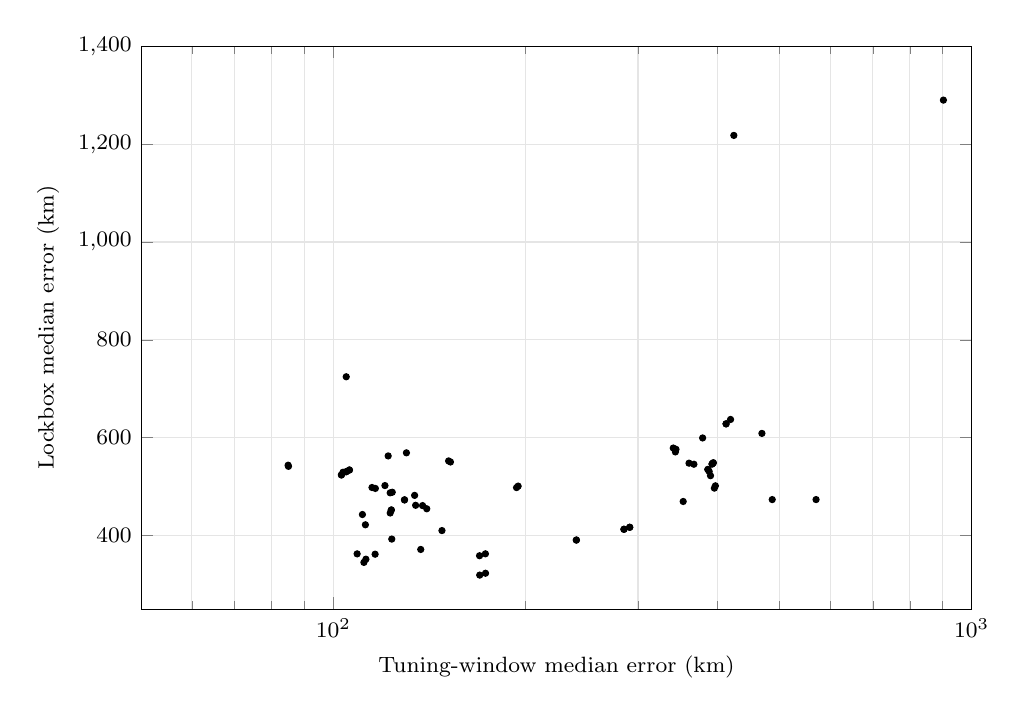
\begin{tikzpicture}
\begin{axis}[
  width=\columnwidth, height=0.72\columnwidth,
  xlabel={Tuning-window median error (\si{\km})},
  ylabel={Lockbox median error (\si{\km})},
  xmin=50, xmax=1000, ymin=250, ymax=1400,
  xmode=log, log basis x=10,
  grid=both, grid style={gray!20},
  tick label style={font=\footnotesize},
  label style={font=\footnotesize},
]
\addplot[only marks, mark=*, mark size=1.1pt, draw=black, fill=black] coordinates {
(84.9,543.9) (85.0,541.6) (102.9,524.1) (102.9,524.1) (103.5,529.3) (103.5,529.2)
(104.7,530.7) (104.7,530.7) (104.7,724.6) (105.9,534.1) (105.9,534.1) (108.9,362.8)
(111.0,443.2) (111.6,345.4) (112.2,422.2) (112.4,351.9) (114.9,498.4) (116.2,362.1)
(116.3,496.5) (120.4,502.3) (121.8,562.9) (122.7,446.3) (122.7,487.5) (123.2,452.4)
(123.2,452.4) (123.4,393.0) (123.6,488.7) (129.2,473.1) (129.2,473.1) (130.1,569.2)
(134.0,482.3) (134.5,462.0) (137.0,371.8) (137.9,461.4) (140.0,454.9) (147.9,410.4)
(151.5,552.7) (152.5,550.5) (169.4,359.0) (169.5,319.4) (173.0,362.9) (173.1,323.2)
(193.6,498.2) (194.7,501.2) (240.2,391.0) (240.2,391.0) (285.2,413.0) (285.2,413.0)
(291.2,417.1) (291.2,417.1) (340.8,579.0) (343.4,571.1) (344.1,576.4) (353.2,469.8)
(360.7,548.1) (367.1,545.9) (378.9,599.6) (386.1,535.2) (386.1,535.2) (388.0,531.1)
(389.8,522.5) (392.0,546.4) (392.0,546.4) (393.7,548.8) (393.7,548.8) (395.3,497.1)
(396.8,501.8) (412.3,628.4) (412.3,628.4) (419.0,637.4) (424.0,1217.7) (469.2,608.9)
(487.0,473.7) (570.5,473.7) (903.2,1289.8)
};
\end{axis}
\end{tikzpicture}
\caption{Every pipeline variant I built ($n=75$), scored on the window I tuned
on (horizontal) and on the held-out window (vertical). If tuning-window skill
transferred, the cloud would run along the diagonal. Spearman
$\rho=+0.30$.}
\label{fig:transfer}
\end{figure}

\subsection{The filters do not know they are wrong}
Coverage is where the failure is least ambiguous. In Table~\ref{tab:head} the
published configuration attains $22\%$ $1\sigma$ coverage on the tuning window
and $9\%$ on the lockbox, against a nominal $68\%$. In the lockbox it reports a
median standard deviation of $201$\,\si{\km} while being wrong by
$532$\,\si{\km} --- roughly a $2.6\sigma$ systematic offset, sustained over 30
days, reported as if it were a $1\sigma$ situation.

Under-coverage this severe is not a tuning problem. A filter whose process noise
is merely too small produces errors that are too large relative to its variance
in a random direction. Here the error has a consistent sign in latitude, which
points at the measurement model rather than at the filter.

\subsection{A matched comparison of EKF, UKF and PF}
\label{sec:matched}
The particle filter beats the Kalman filters in Table~\ref{tab:main}, but it
also differs from them in two ways at once: it uses a Student-$t$ likelihood and
it enforces the feasibility box. Table~\ref{tab:ablate} separates these by
running all four combinations through the same particle filter code path.

The heavy tails are worth $101$\,\si{\km}; the box is worth $9$\,\si{\km}. A
Gaussian particle filter is $84$\,\si{\km} \emph{worse} than the EKF, despite
representing the posterior far more faithfully than a covariance can. So the
honest statement is not that the particle filter beats the Kalman filters. It is
that a Student-$t$ likelihood beats a Gaussian one, and either filter can have
that. The non-Gaussian posterior was not the point.

\begin{table}[t]
\caption{Matched ablation of the particle filter's advantage. Three seeds at
$20{,}000$ particles, all rows through the same code path on the same events.}
\label{tab:ablate}
\centering
\begin{tabular}{lrrr}
\toprule
Configuration & All & Tune & Lock \\
\midrule
PF, Student-$t$ $\nu=4$, box     & $321.2$ & $238.3$ & $395.9$ \\
PF, Student-$t$ $\nu=4$, no box  & $330.2$ & $273.7$ & $396.4$ \\
PF, Gaussian, box                & $413.7$ & $384.1$ & $460.5$ \\
PF, Gaussian, no box             & $430.9$ & $389.8$ & $478.7$ \\
\midrule
EKF                              & $347.2$ & $285.2$ & $413.0$ \\
UKF                              & $356.6$ & $291.2$ & $417.1$ \\
\bottomrule
\end{tabular}
\end{table}

\section{Diagnosis}
\subsection{The residual at the true position}
Because the Argos fixes exist, I can do something better than inspect filter
output: I can evaluate the measurement model at the \emph{true} position. For
each twilight event with an Argos fix within $8$ hours ($63$ of $228$ events), I
compute the predicted twilight time at the interpolated true position and
subtract the observed one. This isolates measurement-model error from filter
error completely.

Table~\ref{tab:resid} gives the result by half-month. Two features matter. The
branch-corrected residual $y$ sits near $+34$ minutes from the first half of
March onwards, which is five to six times the model's own $\sigma$; and the two
twilight branches move in \emph{opposite} directions, with lockbox medians of
$+12$ minutes at dawn and $-71$ minutes at dusk.

The antisymmetry is the diagnostic. A clock error, or a drift in the tag's time
base, would shift both branches the same way. An antisymmetric shift compresses
the apparent day length, and day length is exactly what carries latitude. At
this time of year about $60$ minutes of day-length error is worth roughly
$650$\,\si{\km} of latitude, which matches the size and the sign of the lockbox
latitude bias of $-413$ to $-543$\,\si{\km} measured in Table~\ref{tab:ladder}.

So the model was not slightly wrong at the end of the deployment. It was wrong
by five to six of its own sigmas for the whole record, and the lockbox merely
made that visible.

\begin{table}[t]
\caption{Branch-corrected twilight residual at the true position, by half-month.
$y$ is in minutes, depth in \si{\m}, and $|z|$ is the residual in units of the
model's own $\sigma$.}
\label{tab:resid}
\centering
\begin{tabular}{lrrrr}
\toprule
Half-month & $n$ & $y$ & depth & $|z|$ \\
\midrule
2008-02a &  1 & $-10.3$ &  88 & $2.9$ \\
2008-02b &  9 & $-10.1$ &  48 & $5.0$ \\
2008-03a &  7 & $+34.9$ &  51 & $6.1$ \\
2008-03b &  7 & $+33.9$ &  13 & $5.9$ \\
2008-04a &  6 & $+34.8$ &  50 & $6.1$ \\
2008-04b &  9 & $+33.9$ &  41 & $5.9$ \\
2008-05a & 11 & $+55.0$ &  56 & $9.6$ \\
2008-05b &  6 & $+27.7$ &  94 & $5.7$ \\
2008-06a &  7 & $+13.5$ &  92 & $3.8$ \\
\midrule
Tuning   & 51 & $+34.2$ &  49 & --- \\
Lockbox  & 12 & $+27.5$ &  98 & --- \\
\bottomrule
\end{tabular}
\end{table}

\subsection{Depth of detection, and an unidentifiable parameter}
The depth at which a twilight is recorded is the obvious candidate mechanism:
light attenuates with depth, so a tag deeper in the water column crosses any
fixed irradiance threshold later at dawn and earlier at dusk --- antisymmetric,
as observed.


\begin{figure}[t]
\centering
\includegraphics[width=\columnwidth]{figs/03_twilight_depths}
\caption{Depth at which each twilight was recorded, through the deployment. The
calibration window reaches \SI{94}{\m} at the 95th percentile; the lockbox
reaches \SI{182}{\m}. The depth term in \eqref{eq:h0} is fitted entirely inside
the shallower range.}
\label{fig:depths}
\end{figure}

The depth distribution differs sharply between windows. In the calibration
window the median twilight depth is $51$\,\si{\m} and the 95th percentile is
$94$\,\si{\m}; in the lockbox the median is $98$\,\si{\m} and the 95th percentile
is $182$\,\si{\m}. The parameter $\beta$ in \eqref{eq:h0} was therefore fitted
over a range of depths that the lockbox almost entirely exceeds.

Quantitatively the mechanism is consistent but weakly evidenced. Regressing
$y$ on $\log(1+z)$ over the non-lockbox events gives
$y \approx 8.8 + 4.9\log(1+z)$, and extrapolating that to the lockbox median
depth of $98$\,\si{\m} predicts $+31.5$ minutes against $+27.5$ observed. The
magnitude is right. But the rank correlation itself is weak and not significant
($\rho=+0.27$, $p=0.05$, $n=51$), so I would call the mechanism consistent with
the data rather than established by it.

The sharper statement is about identifiability. Fitted on the raw-light twilight
times, $\beta$ comes out at $+0.0085$ per log-metre, essentially zero. Fitted on
the LightLoc times, the same physical quantity comes out at $+0.89$. Two orders
of magnitude apart. No goodness-of-fit diagnostic in the calibration window
flags this, because the calibration window does not span enough depth to
constrain $\beta$ at all. A support check does flag it, and costs nothing.

\subsection{A recalibration that made things worse}
\label{sec:recal}
This is the single most useful negative result here, and the easiest to state.

Refitting \eqref{eq:h0} on the raw-light twilight times cuts the
calibration-window residual RMS to $4.80$ minutes, against per-branch standard
deviations of $12.88$ and $10.43$ minutes for the original LightLoc calibration.
By every calibration-window diagnostic it is a large improvement.

Held out, it is a large regression. On identical events, the identical filter and
the identical seed, the refitted constants give $364.4$\,\si{\km} median error on
the evaluation window where the original constants give $124.3$\,\si{\km}. A
recalibration that more than halves the residual it was fitted to makes
out-of-sample accuracy roughly three times worse.

The mechanism is the one above: the refit buys its low residual by driving
$\beta$ to zero, which is defensible inside a window spanning $0$--$94$\,\si{\m}
and indefensible in a window reaching $182$\,\si{\m}. The general lesson is that
a sensor-error model fitted on a window that does not span the operating range of
its own regressors will look well calibrated on that window and fail silently
outside it.

A practical note belongs here too. In the notebook these constants live at module
scope and are installed by a context manager, because the first version of this
audit ran the raw-light filters outside that scope and silently used the wrong
constants --- producing numbers that looked three times better than they were.
The audit now begins with an equivalence test asserting that the bias-state
filter with $\sigma_b=0$ reproduces the published filter to within seed noise
($-8.3$ and $-6.4$\,\si{\km} on the two readouts). Global mutable calibration
state is a reproducibility hazard, and a cheap assertion catches it.

\section{A Fix Chosen Without the Lockbox}
\label{sec:fix}
The diagnosis says the threshold is biased and antisymmetric. Rather than try to
predict that bias offline --- which Section~\ref{sec:recal} shows is exactly
where the previous attempt failed --- the filter can estimate it online. I add
one scalar to the state, a threshold bias $b$ in minutes entering the
observation as $+b$ at dawn and $-b$ at dusk, evolving as a random walk with
scale $\sigma_b$ per $\sqrt{\text{day}}$. The state becomes
$[\varphi,\lambda,v_E,v_N,b]$. This adds one hyperparameter and no new data.

\subsection{Selecting $\sigma_b$ honestly}
$\sigma_b$ is chosen by maximising the filter's own marginal likelihood
accumulated over the tuning window only. Table~\ref{tab:sigb} shows the sweep.
The evidence criterion selects $\sigma_b=3$. For comparison, a rule that matched
tuning-window coverage to nominal would have selected $\sigma_b=1$, and the
value that is actually best on the lockbox is $\sigma_b=5$ --- which the
evidence rule did not pick, as it should not, having never seen the lockbox.

Of the six non-zero values, all six beat $\sigma_b=0$ on tuning-window evidence,
two beat it on lockbox median error, and two beat it on lockbox coverage. The
evidence criterion reliably prefers a bias state; the held-out data does not
reliably reward one.

\begin{table}[t]
\caption{Selecting the threshold-bias random-walk scale by tuning-window
marginal likelihood. Three seeds at $20{,}000$ particles. The lockbox columns
were printed after the selection was made and played no part in it.}
\label{tab:sigb}
\centering
\begin{tabular}{rrrrrr}
\toprule
$\sigma_b$ & $\log Z_\text{tune}$ & Tune & cov$_\text{T}$ & Lock & cov$_\text{L}$ \\
\midrule
$0$  & $-1176.2$ & $315.6$ & $27\%$ & $538.8$ & $15\%$ \\
$1$  & $-1087.7$ & $260.6$ & $49\%$ & $650.2$ & $3\%$ \\
$2$  & $-1069.5$ & $330.9$ & $40\%$ & $462.2$ & $28\%$ \\
$3$  & $\mathbf{-1060.0}$ & $389.8$ & $33\%$ & $567.8$ & $10\%$ \\
$5$  & $-1061.8$ & $324.4$ & $34\%$ & $423.6$ & $18\%$ \\
$8$  & $-1070.3$ & $414.8$ & $27\%$ & $589.0$ & $5\%$ \\
$12$ & $-1073.3$ & $427.1$ & $18\%$ & $720.3$ & $5\%$ \\
\bottomrule
\end{tabular}
\end{table}

\subsection{What the fix buys, and what it does not}
Table~\ref{tab:head} gives the honest answer at full particle count over ten
seeds. Adding the bias state moves tuning-window $1\sigma$ coverage from $22\%$
to $38\%$, a real and reproducible gain. It leaves the full-window error
unchanged ($+12.3$\,\si{\km}, $1.1$ standard errors), leaves tuning-window error
unchanged ($-5.3$\,\si{\km}, $0.5$ standard errors), and makes lockbox error
\emph{worse} ($+83.0$\,\si{\km}, $2.7$ standard errors). Lockbox coverage stays
flat at $8$--$9\%$.

So the fix is the right response to the diagnosis, it is selected without
touching held-out data, and it does not generalise. I am reporting it because it
failed. Had I selected $\sigma_b$ on the lockbox I could have reported
$423.6$\,\si{\km} and a $109$\,\si{\km} improvement, and it would have been
meaningless.

Table~\ref{tab:ladder} puts the fix beside the two alternatives one would
naturally reach for. Inflating the twilight $\sigma$ improves the tuning window
substantially ($316 \rightarrow 165$\,\si{\km} at $3\times$) and does nothing out
of sample, which is itself the signature of a bias rather than of
under-dispersed noise. Rejecting deep twilights is actively harmful: it removes
exactly the large-residual events that were inflating the variance, so the
filter becomes more confident and less accurate at once, with lockbox coverage
falling to zero. Every row retains a lockbox latitude bias of at least
$413$\,\si{\km}. None of these is a fix.

\begin{table}[t]
\caption{Candidate responses to the diagnosis, three seeds at $20{,}000$
particles. $\bar{s}_\text{L}$ is the median reported standard deviation and
$\Delta\varphi_\text{L}$ the median latitude bias, both in the lockbox.}
\label{tab:ladder}
\centering
\begin{tabular}{lrrrrr}
\toprule
 & Tune & Lock & cov$_\text{L}$ & $\bar{s}_\text{L}$ & $\Delta\varphi_\text{L}$ \\
\midrule
As published            & $315.6$ & $538.8$ & $15\%$ & $219$ & $-413$ \\
Twilight $\sigma\times2$ & $220.5$ & $528.4$ & $15\%$ & $190$ & $-473$ \\
Twilight $\sigma\times3$ & $164.6$ & $555.9$ & $5\%$  & $206$ & $-548$ \\
Depth QC, $z\le94$\,\si{\m} & $478.1$ & $978.6$ & $0\%$ & $178$ & $-863$ \\
Bias state, $\sigma_b=2$ & $330.9$ & $462.2$ & $28\%$ & $196$ & $-424$ \\
Bias state, $\sigma_b=3$ & $389.8$ & $567.8$ & $10\%$ & $176$ & $-543$ \\
Depth QC $+$ bias state  & $460.1$ & $921.5$ & $0\%$  & $214$ & $-838$ \\
\bottomrule
\end{tabular}
\end{table}

\section{Discussion}
\subsection{What survives}
A Student-$t$ twilight likelihood is worth about $100$\,\si{\km} and is the
largest single modelling win in this work --- considerably more than the choice
of filter, which is worth about $26$\,\si{\km}. Smoothing beats filtering
consistently for all three estimators. Independent aiding is what breaks the
equinox degeneracy: SST cuts March error from $522$ to $109$\,\si{\km}, because
its information is orthogonal to day length rather than because it is more
accurate. And once a hard constraint makes the posterior multimodal, the readout
stops being innocent: the same particle cloud reads $364$\,\si{\km} at the
posterior mean and $452$\,\si{\km} at the local MAP.

\subsection{What does not}
The headline, as a measure of accuracy. The ablation ladder, which was built
below the seed-noise floor. The raw-light recalibration, which improved the
quantity it was fitted to and tripled the held-out error. And the bias-state fix,
as an accuracy claim.

\subsection{Limitations}
This is one animal, one deployment, and one ground-truth track. The lockbox
contains $20$ matched events, so lockbox medians carry wide intervals --- the
seed standard deviation alone is $90$\,\si{\km}, and sampling error on $20$
events is comparable. Nothing here should be read as a general ranking of
nonlinear filters; it is a statement about what this data set can resolve, which
is less than I originally claimed. The Argos error model for classes 0, A and B
is assumed rather than known. GPE3 is a black box, so I can say that it
generalises better but not why.

\subsection{What I would do differently}
Hold out a block of ground truth before writing any model code --- a block at the
end, scored once. Report seed variance on every stochastic result and refuse to
interpret any difference smaller than it; two seeds would have killed most of the
ladder. And treat calibration support as a first-class check: for every fitted
sensor parameter, compare the range of its regressors in the calibration window
against the range expected at deployment. A goodness-of-fit plot cannot show you
an unidentifiable parameter; a support check can.

\section{Conclusion}
Light-level geolocation of this record is dominated not by the choice of
nonlinear filter but by a biased measurement model that no filter in the family
can detect from the data it is given. On the window I tuned on, my best
configuration reaches $117$\,\si{\km} and approaches the manufacturer's
smoother. On 30 days I never looked at, it reaches $544$\,\si{\km} against the
smoother's $118$\,\si{\km}, and reports a $201$\,\si{\km} standard deviation
while being wrong by $532$\,\si{\km}.

The measurable contributions are therefore negative, and I think more useful than
the positive claims they replace. Seed-to-seed spread of $29$--$90$\,\si{\km}
invalidates an ablation ladder built from $1$--$5$\,\si{\km} steps.
Tuning-window rank predicts held-out rank only weakly ($\rho=+0.30$), so the
best-on-tuning variant ranks $54$th of $75$ out of sample. A recalibration that
halved its own fitting residual tripled held-out error, because the parameter it
adjusted was never identifiable from the calibration window. And a principled
one-parameter fix, chosen without ever touching the held-out data, improved
calibration and not accuracy.

The estimator that generalises here is the one I did not write. The part of this
work I would defend is the protocol that let me find that out.

\section*{Reproducibility}
Everything runs top to bottom in a single Colab notebook with no manual steps.
The tag archives are fetched at run time from the ATN Data Assembly Center by
stable UUID, so a cold start gets byte-identical inputs; the raw data are not
redistributed. All seeds are fixed in code. Particle counts are stated with every
result: Table~\ref{tab:head} uses $120{,}000$ particles over ten seeds, and
Tables~\ref{tab:ablate}, \ref{tab:sigb} and \ref{tab:ladder} use $20{,}000$
particles over three seeds. Absolute values are therefore not comparable
\emph{between} those two groups, although every comparison \emph{within} a
table is like-for-like. Table~\ref{tab:main} reports each configuration at the
particle count at which it was built.
Figures are regenerated by the notebook. Code, the technical report and build
instructions are at
\url{https://github.com/vivianesolomon/pat-tag-geolocation}.
Environment: Python 3.13, NumPy 2.1.3, SciPy 1.16.3, pandas 2.2.3,
Matplotlib 3.10.0, netCDF4 1.7.4.

\section*{Acknowledgment}
Tag data are published through the Animal Telemetry Network Data Assembly Center.
The GPE3 reference tracks were produced by the tag manufacturer's software.
\end{document}
